% !TEX TS-program = pdflatexmk
%header and footer for separate chapter files

\ifx\whole\undefined
\documentclass[12pt, leqno]{book}
\usepackage{graphicx}
\input style-for-curves.sty
\usepackage{hyperref}
\usepackage{showkeys} %This shows the labels.
%\usepackage{SLAG,msribib,local}
%\usepackage{amsmath,amscd,amsthm,amssymb,amsxtra,latexsym,epsfig,epic,graphics}
%\usepackage[matrix,arrow,curve]{xy}
%\usepackage{graphicx}
%\usepackage{diagrams}
%
%%\usepackage{amsrefs}
%%%%%%%%%%%%%%%%%%%%%%%%%%%%%%%%%%%%%%%%%%
%%\textwidth16cm
%%\textheight20cm
%%\topmargin-2cm
%\oddsidemargin.8cm
%\evensidemargin1cm
%
%%%%%%Definitions
%\input preamble.tex
%\input style-for-curves.sty
%\def\TU{{\bf U}}
%\def\AA{{\mathbb A}}
%\def\BB{{\mathbb B}}
%\def\CC{{\mathbb C}}
%\def\QQ{{\mathbb Q}}
%\def\RR{{\mathbb R}}
%\def\facet{{\bf facet}}
%\def\image{{\rm image}}
%\def\cE{{\cal E}}
%\def\cF{{\cal F}}
%\def\cG{{\cal G}}
%\def\cH{{\cal H}}
%\def\cHom{{{\cal H}om}}
%\def\h{{\rm h}}
% \def\bs{{Boij-S\"oderberg{} }}
%
%\makeatletter
%\def\Ddots{\mathinner{\mkern1mu\raise\p@
%\vbox{\kern7\p@\hbox{.}}\mkern2mu
%\raise4\p@\hbox{.}\mkern2mu\raise7\p@\hbox{.}\mkern1mu}}
%\makeatother

%%
%\pagestyle{myheadings}

%\input style-for-curves.tex
%\documentclass{cambridge7A}
%\usepackage{hatcher_revised} 
%\usepackage{3264}
   
\errorcontextlines=1000
%\usepackage{makeidx}
\let\see\relax
\usepackage{makeidx}
\makeindex
% \index{word} in the doc; \index{variety!algebraic} gives variety, algebraic
% PUT a % after each \index{***}

\overfullrule=5pt
\catcode`\@\active
\def@{\mskip1.5mu} %produce a small space in math with an @

\title{Personalities of Curves}
\author{\copyright David Eisenbud and Joe Harris}
%%\includeonly{%
%0-intro,01-ChowRingDogma,02-FirstExamples,03-Grassmannians,04-GeneralGrassmannians
%,05-VectorBundlesAndChernClasses,06-LinesOnHypersurfaces,07-SingularElementsOfLinearSeries,
%08-ParameterSpaces,
%bib
%}

\date{\today}
%%\date{}
%\title{Curves}
%%{\normalsize ***Preliminary Version***}} 
%\author{David Eisenbud and Joe Harris }
%
%\begin{document}

\begin{document}
\maketitle

\pagenumbering{roman}
\setcounter{page}{5}
%\begin{5}
%\end{5}
\pagenumbering{arabic}
\tableofcontents
\fi


\chapter{Scrolls and the Curves They Contain}
\label{ScrollsChapter}


\begin{verbatim}
 The naming of cats is a difficult matter,
 It isn't just one of your everyday games.
 You may think that I am as mad as a hatter,
 When I tell you each cat must have three different names.
 The first is the name that the family use daily ...
 But I tell you, a cat needs a name that's particular ...
 But above and beyond there's still one name left over,  ...
 [his] deep and inscrutable, singular name.
\end{verbatim}
--T. S. Eliot, Old Possum's Book of Practical Cats\footnote{\cite{PracticalCats}}

\section*{}
Some of the simplest subvarieties in projective space are the \emph{rational normal scrolls}. They appear in many contexts in algebraic geometry, and are useful for describing the embeddings of curves of low degree and genus. 

Like the cats in T. S. Eliot's poem, scrolls can be seen from three rather different points of view, each useful in a different context: First a classical geometric construction, then an algebraic description that allows one to ``find" the scrolls containing a given variety, and then a more modern geometric definition that makes it easy to understand the divisors on a scroll. Finally, we turn to some of the applications to the embeddings of curves. We will focus on the 2-dimensional case because this is the case that occurs in our applications.

In this chapter we will refer to rational normal scrolls simply as scrolls. The third characterization we will give lends itself to a natural generalization to  irrational ruled varieties, In the literature the word ``scroll'' is often used for this wider class.

\section{Some classical geometry}\label{daily name}

To construct a scroll of dimension 2 in $\PP^n$, we start by choosing integers $0\leq a_1 \leq a_2$ with $a_1 + a_2 = n-1$, and consider  a pair of complementary linear subspaces $\PP^{a_1}$ and $\PP^{a_2} \subset \PP^n$---that is, we express an $(n+1)$-dimensional vector space as a direct sum $ V_1 \oplus V_2$ of subspaces $V_1, V_2 \subset V$ of dimensions $a_1+1$ and $a_2+1$, and let $\PP^{a_1} = \PP V_1$ and $\PP^{a_2} = \PP V_2 \subset \PP (V_1\oplus V_2)$.

Next, for $i=1,2$, we take $\phi_i : \PP^1 \to \PP^{a_i}$ to be the parametrization of the rational normal curve of degree $a_i$ given by a basis of homogeneous polynomials of degree $a_i$ (if $a_i = 0$ this is just the constant map from $\PP^1$ to a point.) Finally, we define the scroll $S(a_1, a_2)$ to be the union of the lines
$$
S(a_1,a_2) := \bigcup_{p\in \PP^1} \overline{\phi_1(p), \phi_2(p)}.
$$

We call the curve $C_{a_{1}}$ the \emph{directrix} of the scroll, and we call the lines $ \overline{\phi_1(p), \phi_2(p)}$ the \emph{rulings} of the scroll. For example we can realize a smooth quadric surface in $\PP^3$ as the union $S(1,1)$ of the lines joining corresponding points on two skew lines. 

\fix{Insert picture!}

In the degenerate case $a_{1}= 0$, the surface $S(0,a_{2})$ is the cone
in $\PP^{a_{2}+1}$ over a rational normal curve of degree $a_{2}$. Since $S(0,a_2)$ is singular when $a_2\geq 2$, it is useful to consider the surface
$$
\tilde S(0, a_2) := \left\{ (t, q) \in \PP^1 \times \PP^n  \mid q \in \overline{\phi_1(t), \phi_2(t)}\right)\}.
$$
This is the blow-up of the cone $S(0, a_2)$ at its vertex; like the surfaces $S(a_1,a_2)$ with $a_1 > 0$ it is a $\PP^1$ bundle over $\PP^1$ and thus is smooth. As we shall see, $\tilde S(0, a_2)$ is isomorphic to the scroll $S(1, a_2+1)$.

It is not hard to prove directly that $S(a_1,a_2)$ is an algebraic variety, and we shall soon write down its defining equations.

From the description above we can immediately deduce the dimension and degree of a scroll:

\begin{proposition}
\begin{enumerate}
\item $S(a_1,a_2)$ is a nondegenerate surface.
 \item $S(a_1,a_2)$ has degree $a_1+a_2$, and codimension $a_1+a_2-1.$
 \item $S(a_{1},a_{2})$ is non-singular if $a_{1}>0$.
 \end{enumerate}
\end{proposition}\label{deg and codim}

\begin{proof}
 The rational normal curves separately span the spaces $\PP^{a_i}$, so a hyperplane containing both of them would contain $\overline{\PP^{a_1}, \PP^{a_{2}}} = \PP$, proving nondegeneracy. 
 
 It is clear from our description that $S$ is 2-dimensional, and thus of
codimension $a_{1}+a_{2}+1 -2 = a_{1}+a_{2}-1$. 

To compute the degree, we choose a general hyperplane $H$ containing $\PP^{a_{1}}$. The intersection $H\cap C_{2}$ consists of $a_{2}$ reduced points. Thus the intersection $H\cap S$ consists of $C_{1}$ and the $a_{2}$ reduced lines connecting 
the points of $H\cap C_{2}$ with their corresponding points on $C_{1}$; this union has degree $a_{1}+a_{2}$.

If $0< a_{1}$ we also see from this argument that, given any point  $p\in S(a_{1},a_{2})$, there is
a hyperplane section that is non-singular at $p$, and thus $S(a_{1},a_{2})$ is nonsingular at $p$.
\end{proof}

A completely parallel construction creates rational normal scrolls of dimension $r$. Start with a series of integers $0 \leq a_1 \leq \dots \leq a_r$;
set $N = \sum_{i=1}^{r}(a_{i}+1)$,  and
decompose $\CC^{N}$ as
$$
\CC^{N} = \bigoplus_{i=1}^{r}\CC^{a_{i}+1}.
$$
Let $\PP^{a_{i}}\subset \PP^{N-1}$ be the subspaces corresponding to the summands,  choose
maps $\phi_i : \PP^1 \to \PP^{a_{i}}$ be a map given by a basis of homogeneous polynomials of degree $a_i$, and define the scroll $S \subset \PP^{N-1}$ by
$$
S:=S(a_{1}, \dots, a_{r}) = \bigcup_{p\in C_{1}}\overline{\phi_1(p), \phi_{2}(p), \dots, \phi_{r}(p)}.
$$
The variety $S$ is nondegenerate of codimension $N-1-r$ and degree $\sum a_{i} = N-r$. The proof is similar to the one we gave for $r=2$.

%As in the surface case, if one or more of the indices $a_i$ are equal to 0, the resulting variety $S$ is a cone. In these cases, it is again useful in some settings to introduce the blow-up of this cone along its vertex, which we can realize as the variety
%$$
%\tilde S := \left\{ (t, q) \in \PP^1 \times \PP^n  \mid q \in \overline{\phi_1(t), \dots, \phi_r(t)}\right)\}.
%$$

To put this construction in context, we recall an elementary fact of projective geometry:
 
\begin{proposition}\label{minimal degree}
 Any irreducible, nondegenerate variety $X$ of codimension $c$ in $\PP^{N}$ has degree $\geq c +1$.
\end{proposition}

\begin{proof} We do induction on $\dim X$. If $H\cong \PP^{N-1}\subset \PP^N$ is a hyperplane then $H\cap X$ spans
$H$ by Proposition~\ref{arbitrary hyperplane}. Bertini's Theorem shows that if $H$ is a general hyperplane then $H\cap X$ is either an irreducible variety of 
(if $\dim X\geq 2$) or a set of reduced points. In the former case we are done by induction. In the latter case
we appeal to the fact that fewer than $c+1$ points could not span $\PP^c$.
 \end{proof}

Thus scrolls are \emph{varieties of minimal degree}. The reader already knows that the rational normal curves of degree $a$ in $\PP^{a}$ are the only irreducible, nondegenerate curves of degree $a$ and codimension $a-1$. A celebrated theorem of del Pezzo (for surfaces) and Bertini (in general) generalizes this statement:

\begin{fact}\label{classification of scrolls} 
Any irreducible, nondegenerate variety $X\subset \PP^{N}$  with $\deg X = \codim X+1$ is either a quadric hypersurface, a scroll, the Veronese surface in $\PP^{5}$ or a cone over the Veronese surface.
\end{fact}

A proof may be found in \cite{Eisenbud-Harris-Centennial}.

One interesting way to view the construction of a scroll is that we chose subvarieties $C_{i}\subset \PP^{a_{i}}$ and a one-to-one correspondence between them, that is, a subscheme
$\Gamma\subset \prod C_{i}$ that projects isomorphically onto each $C_{i}$; the scroll is then the
union of the planes spanned by sets of points $p_{i}\in C_{i}$ that are ``in correspondence''. There are other interesting varieties constructed starting with other choices of subvarieties $C_{i}$ and subschemes---not necessarily reduced---of $\prod C_{i}$. See \cite{Eisenbud-Sammartano} for an exploration of this idea.

We tend to speak of ``the'' rational normal scroll rather than ``a'' rational normal scroll'', despite the choices made in the definition, for the following reason:

\begin{proposition}\label{uniqueness of scrolls}
The scroll $S(a_1,a_2)$ is, up to a linear automorphism of $\PP^{a_1+a_2+1}$, independent of the choices made in its
 definition. 
\end{proposition}

\begin{proof} 
To simplify the notation, set $S := S(a_{1}, a_{2})$ and $\PP := \PP^{a_1+a_2+1}$.
To construct $S$ we chose 
\begin{enumerate}
 \item disjoint subspaces $\PP^{a_i}\subset \PP$;
 \item a rational normal curve in each subspace; and
 \item an isomorphism between these curves.
\end{enumerate}
Elementary linear algebra shows that there are automorphisms of $\PP$ carrying any choice of disjoint subspaces to any other choice. Further, since the rational normal curve of degree $a$ is unique up to an automorphism of $\PP^{a}$, the choice in (2) can be undone by a linear automorphism. Finally, any automorphism of $C_{a_{2}}\cong \PP^{1}$ extends to an automorphism of $\PP^{a_{2}} = |\cO_{\PP^{1}}(a_{2})|$, and this extends to an automorphism of $\PP$ fixing $\PP^{a_{1}}$ pointwise,
showing that $S(a_{1}, a_{2})$ is independent, up to an automorphism of the ambient space, of the choice in (3)  as well.
\end{proof}



\section{1-generic matrices and the equations of scrolls}\label{particular name}

Suppose that a scheme $X $ is embedded in $\PP^n$ by a complete linear series, and that
$\sO_X(1)$ can be ``factored'' as a tensor product $\sL\otimes \sM$ of invertible sheaves on $X$. If we pick sets of $p$ independent elements $\{\ell_i\}\subset H^0(\sL)$ and  $q$ independent elements $\{m_i\} \subset H^0(\sM)$ then the multiplication map 
$$
\mu: H^0(\sL) \otimes H^0(\sM) \to H^0(\sO_{\PP^n}(1))
$$
 gives rise to 
a $p\times q$ matrix $M_\mu$ of linear forms on $\PP^n$ whose $i,j$ entry is $\mu(\ell_im_j)$.
More abstractly, this is a linear space of matrices obtained from the ``adjunction'' isomorphism 
$\Hom(A\otimes B, C)\cong \Hom(A, \Hom(B,C))$.

Regarding the sections of invertible sheaves as sheaves of functions on $X$, we see from the commutativity of
multiplication that the $2\times 2$ minors
of 
$$
\det \begin{pmatrix}
\ell_{i_1}m_{j_1} & \ell_{i_1}m_{j_2}\\
\ell_{i_2}m_{j_1} &\ell_{i_2}m_{j_2}  
\end{pmatrix},
$$
vanish on $X$---that is, the ideal of $2\times 2$ minors $I_2(M_\mu)$ is contained in the homogeneous ideal
of $X$. 
We will see that, if $p=2$, then the ideal $I_2(M_\mu)$
is the ideal of a rational normal scroll of codimension $q-1$.

For example, the rational normal curve $C_a\subset \PP^a$ is $X = \PP^1$ embedded by the complete
linear series $|\sO_{\PP^n}(a)|$, and $\sO_{\PP^1}(a) = \sO_{\PP^1}(1)\otimes \sO_{\PP^1}(a-1)$.
If we take bases $s^it^j$ in each of $H^0(\cO_{\PP^1}(1))$ and  $H^0(\cO_{\PP^1}(a))$ and use the parametrization
$x_i = s^it^{a-i}$ we get
the $2\times a$ matrix
$$
M_\mu := 
\begin{pmatrix}
x_0&x_1&\dots&x_{a-1}\\
x_1&\dots&x_{a-1}&x_a
\end{pmatrix}.
$$
When restricted to $\PP^1$, this becomes
$$
M_a = \bordermatrix{
& s^{a-1}&s^{a-2}t&\dots&t^{a-1}\cr
s&  s^{a}& s^{a-1}t&\dots&st^{a-1}\cr
t&  s^{a-1}t& s^{a-2}t^{2}&\dots&t^{a}\cr
}$$
where we have written $s,t$ for the basis of $H^0(\sO_{\PP^1}(1))$, and bordered the matrix
with the corresponding bases of $H^0(\sO_{\PP^1}(1))$ and $H^0(\sO_{\PP^1}(a-1))$, and it is obvious
that the minors of $M_a$ are 0.

By a \emph{generalized row} of $M_{a}$, we mean a $\CC$-linear combination of the given rows of $M_{a}$. Note that the points at which the $2\times 2$ minors of $M_{a}$ vanish are the points at which the evaluations of the two rows are linearly dependent; that is, the points at which some
generalized row of $M_{a}$ vanishes identically. From Proposition~\ref{RNC generators}, we see that the points of the rational normal curve are exactly the points where all the linear forms in some generalized row
of $M_{a}$ vanish.


The matrix $M_{\mu}$ shares some properties with the generic $p\times q$ matrix:

\begin{definition}
 A matrix of linear forms $M$ is  \emph{1-generic} if every generalized row of $M$
 consists of $\CC$-linearly independent forms.. 
 \end{definition}

 For example, the matrix 
$$
M = \begin{pmatrix}
 x &y\\
 z&x
\end{pmatrix}
$$
over $\CC[x,y,z]$ is  1-generic, since if a row and column transformation produced a 0 the determinant would be a product of linear forms, whereas
$\det M = x^2-yz$ is irreducible. 

On the other hand, the matrix
$$
M' = \begin{pmatrix}
 x &y\\
 -y&x
\end{pmatrix}
$$
over $\CC[x,y]$ is not 1-generic, since
$$
\begin{pmatrix}
1&0\\
-i&1 
\end{pmatrix}
M'
\begin{pmatrix}
 1&0\\
 i&1
\end{pmatrix}
= 
\begin{pmatrix}
 x+iy&0\\
 0&x-iy
\end{pmatrix}
$$
(but note that it would be 1-generic if we restricted scalars to $\RR$---thus the definition depends on the field).

Here is another way of seeing that $M'$ is not 1-generic over $\CC$:

\begin{lemma}\label{variables needed}
  \label{size of 1-generic} There exist 1-generic $p\times q$ matrices of linear forms in $n+1$ variables over $\CC$ if and only if $n\geq p+q$.
In particular, the dimension of the space of linear forms spanned by the entries of a  1-generic matrix $M$ of size $p\times q$ is at least $p+q-1$. Moreover, if this space of linear forms has dimension $>p+q-1$, then the restriction of $M$ to a general hyperplane is still 1-generic.
\end{lemma}
\begin{proof} Consider any map of vector spaces $\mu : A\otimes B \to C$, where we regard $C$ as a 
space of linear forms.
With notation as above, if $\ell_i\otimes m_j\in \ker \mu$, then the $i,j$ entry of $M_\mu$ is 0 and similarly for
any \emph{pure} tensor $\ell\otimes m\in A\otimes B$. Thus $M_\mu$ is 1-generic if and only if the linear subspace
$\ker \mu \subset  A\otimes B$
is disjoint from the set of pure tensors. Under the isomorphism $A\otimes B \cong \Hom (A^*, B)$
the set of pure tensors corresponds to matrices of rank 1, and this set has codimension $(m-1)(n-1) = mn-m-n+1$
in $\Hom(A^*, B)$ (proof: a rank 1 matrix corresponds to the choice of a 1-quotient of $A^*$ and a 1-dimensional subspace
of $B$, thus a point in $\PP^m \times \PP^n$).
Thus
for $\mu$ to correspond to a  1-generic matrix,  we must have $\codim \ker \mu \geq m+n-1$. Since $\codim \ker \mu = \dim \im \mu\subset C$ we see that any 1-generic matrix must involve at least $m-n+1$ variables. 

Furthermore, the restriction of $M_\mu$ to a hyperplane corresponds to the composite homomorphism
$A\otimes B \to C \to C/\langle x \rangle$, or equivalently to the addition of 1 element to $\ker \mu$, and thus
if $M_\mu$ is 1-generic and involves $>m+n-1$ variables, then the restriction to a general hyperplane
is again 1-generic.
\end{proof}

%\begin{proof}
%If we think of a polynomial ring $\CC[z_0,\dots,z_n]$ as the symmetric algebra
%of a vector space $V$ of rank $n+1$, then we may regard a $p\times q$ matrix of
%linear forms $M$ as coming from a map $m: \CC^{p}\otimes \CC^{q}\to V$. The matrix is 1-generic
%if and only if no ``pure'' tensor $r\otimes s$ goes to zero, that is, iff the kernel $K$ of $m$ intersects the cone of
%pure tensors only in 0. The cone of pure tensors is the cone over the Segre embedding of $\PP^{p-1}\times \PP^{q-1}$, 
%and thus has dimension $(p-1)+(q-1)+1$. Thus a general subspace $K$ of codimension $\geq p+q-1$ will intersect the cone
%only in 0, but any larger subspace $K$ will intersect the cone non-trivially,  and the first two statements follow.
%
%Moreover, if $K$ is any space of codimension $>p+q-1$ that intersects the cone only in 0, then the general subspace $K'\subset K$
%of dimension one larger still intersects the cone only in 0, proving the last statement.
%\end{proof}

\begin{proposition}\label{some generators}
Let $X$ be
an irreducible, reduced variety, and suppose that $\sL,\sM$ are invertible sheaves on $X$.
The matrix $M_\mu$ coming from the map $\mu:H^0(\sL) \otimes H^0(\sM) \to H^0(\sL\otimes \sM)$
is 1-generic.
\end{proposition}

\begin{proof} The entries of the generalized row of $M_\mu$ corresponding to $s\in H^0(\sL)$
are a basis of $s\cdot H^0(\sM) \cong H^0(\sM)$, and are thus
linearly independent.
\end{proof}

The 1-generic matrices $M$ of size $2\times a$ have a simple classification. The beginning of the story is the
 calculation of the codimension of the ideal $I_2(M)$ generated by the $2\times 2$ minors of $M$:

\begin{lemma}\label{codim of 2,n 1-generic}
If $M$ is a $2\times a$ matrix of linear forms in $\CC[x_0,\dots, x_n]$, and $M$ is 1-generic, then 
  $V(I_2(M))$ is irreducible of codimension $a-1$.
\end{lemma}

\begin{proof}
The algebraic set defined by $I_2(M)$ is the set of points on which a generalized row $r_\lambda, \ \lambda\in \PP^1$ of $M$ vanishes.
Because $M$ is 1-generic, each $V(r_\lambda)$ has codimension $a$. Thus $V(I_2(M))$ is fibered by projective
spaces of dimension $n-a$ over $\PP^1$, and is thus irreducible of dimension either $n-a$ or $n-a+1$. In the first
case all the spaces $V(r_\lambda)$  would be equal, contradicting Lemma~\ref{variables needed}.
\end{proof}


We have seen in Proposition~\ref{RNC generators} that the ideal of minors of
$$
M_{a}:= 
\begin{pmatrix}
 x_0&x_1&\dots&x_{a-1}\\
 x_1&x_2&\dots&x_{a}\\
\end{pmatrix}
$$ 
generates the ideal of the rational normal curve of degree $a$ in $\PP^a$, and is thus prime. More generally:

\begin{theorem}\label{1-generic basics}  
Let $I = I_2(M)$  be the ideal generated by the $2\times 2$ minors of  a 1-generic, $2\times a$ matrix $M$
of linear forms in $S = \CC[x_0,\dots, x_n]$.
 \begin{enumerate}

\item The ideal $I$ is prime, and $V(I)$ either is smooth, or is a cone over a smooth variety.

\item If $a=n$ then $V(I)$ is a rational normal curve. More generally, the variety $V = V(I) \subset \PP^n$ has degree $a$ and codimension $a-1$ and is thus a variety of minimal degree.
\end{enumerate}
\end{theorem}

\begin{proof}  By Lemma~\ref{codim of 2,n 1-generic} the set that $V(I)$ has codimension $a-1$.

%By Lemma~\ref{variables needed}, the scheme defined by $I$ spans $\PP^a$.

If the span of the linear forms in $M$ is not the whole space of linear forms on $\PP^n$, then $V(I)$ is a cone,
so we may assume that the entries of $M$ generate the maximal ideal.

 Let $p\in V(I)$ be a point, so that $M$ has a generalized row---without loss of generality the second row---whose 
 entries vanish
at $p$. Since not all the linear forms
of $S$ can vanish at a point of $\PP^n$, one of the entries of the first row, say $\ell_{1,1}$ is nonzero
at $p$. By making row and column transformations we may reduce to the case where
$\ell_{1,j}$ vanishes at $p$ for all $j\neq 1$ and also $\ell_{2,1}$ vanishes at $p$. Since all the minors
vanish at $p$, we see that all the entries $\ell_{2,j}$ must vanish at $p$ as well. Since the entries
of each generalized row are linearly independent, the ideal generated by the entries of the second row define a plane of
$\Lambda$ codimension $a$ containing $p$. 

Over the local ring $\sO_{\PP^n, p}$ at $p$ the element $\ell_{1,1}$ becomes a unit.
Thus the element $\ell_{2,j}$ together with the minors 
$$
\det 
\begin{pmatrix}
\ell_{1,1}& \ell_{1,j}\\
\ell_{2,1}& \ell_{2,j}
\end{pmatrix}
$$
for $j\neq 1$ generate the ideal of $\Lambda$ locally at $p$. Since the products
$\ell_{2,1}\ell_{1,j}$ vanish to order 2 at $p$, we see that the zariski tangent space to the scheme $V(I)$
has codimension at most $1$ in $\Lambda$, and thus codimension $\leq a-1 = \codim (V(I))$ in $\PP^n$. It follows that $V(I)$ is smooth at $p$, and since $V(I)$ is
irreducible, the ideal $I$ is prime.

If $a=n$ then $V(I)$ is a smooth, nondegenerate curve. In Chapter~\ref{HomologicalChapter} we will construct the Eagon-Northcott complex $EN(M)$. By Theorem~\ref{EN}, the complex $EN(M)$ is a free resolution,
and if $M'$ is the ideal of the rational normal curve, then $EN(M')$ is again a resolution. Since the Hilbert
function of $V(I)$ can be computed from the free resolution, it follows that $V(I)$ has the same Hilbert function
as $V(I_2(M)$, and thus $V(I)$ is a rational normal curve.

If $a<n$ then by Lemma~\ref{some generators} there is linear form $\ell$ such that $M$ remains 1-generic modulo $\ell$.
Since $I_2(M)$ is prime it has the same degree and codimenion as $I_2(M) +(x)/(x) \subset S/(x)$, so by induction its degree
is $a$.
\end{proof}

We can use Theorem~\ref{1-generic basics} to prove a classic result of Castelnovo, characterizing large sets of 
points on a rational normal curve. It is a key element in Castelnovo's classification of Castelnuovo curves of high
degree, Theorem **** below.

\begin{corollary}(Castelnovo's $2r+3$ Lemma)\label{Castelnuovo2r+3}
If $\Gamma\subset \PP^r$ is a set of $\geq 2r+3$ distinct points in linearly general position, then
$\Gamma$ is contained in a rational normal curve if and only if $\Gamma$ imposes only $2r+1$
conditions on quadrics. 
\end{corollary}
 
 To understand the approach taken in the proof below, recall that in the case of a twisted
 cubic, whose equations are the minors of the matrix
 $$
\begin{pmatrix}
 x_0&x_1&x_2\\
 x_1&x_2&x_3
\end{pmatrix}
 $$
the first column defines a secant line to the twisted cubic, and the two minors involving the first column are a regular sequence defining the union of the twisted cubic and that secant line.
In general a rational normal curve may be defined by the 1-generic matrix coming associated to the product $H^0(\sO_{\PP^1}(1)) \otimes H^0(\sO_{\PP^1}(r-1)) \to H^0(\sO_{\PP^1}(r))$,
and it follows from that description that the columns of the matrix define the $(r-1)$-secant $(r-2)$-planes to the curve. In the proof below we reconstruct the matrix starting from such a secant plane.

\begin{proof}
By Theorem~\ref{1-generic basics} it suffices to construct a 1-generic $2\times r$ matrix $M$ whose minors vanish on
$\Gamma$. Note that the dimension of the space of quadrics on $\PP^r$, which is $\binom{r+2}{2}$, is equal to the sum
$\binom{r}{2}+2r+1$, so the vector space of quadrics containing $\Gamma$ has dimension $\binom{r}{2}$.

Enumerate the points $p_i\in \Gamma$, and let $\Lambda = V(a_1,b_1)$ be the linear
space spanned by $p_1,\dots,p_{r-1}$. 

 The number of
conditions $\Lambda$ imposes on quadrics is $\binom{r}{2}$, but the $r-1$ points of $\Gamma \cap \Lambda$
already impose $r-1$ conditions, so the dimension of the space of quadrics containing $\Lambda\cup \Gamma$
is $\binom{r}{2}-\bigl(\binom{r}{2}-(r-1)\bigr) = r-1.$ These quadrics are contained in the ideal $(a_1,b_1)$, so a
basis for them
may be written as the $2\times 2$ minors that involve the first column of a matrix
$$
M := \begin{pmatrix}
a_1&a_2&\dots&a_{r}\\
b_1&b_2&\dots&b_{r}
\end{pmatrix}.
$$
We will show that $M$ is 1-generic, and that its minors vanish on $\Gamma$, as required.
Note that row and column operations do not change either of these properties.

If $M'$ were not 1-generic then we could perform row and column operations that do not change the 
span of the first column to arrive at a matrix with an entry in some column equal to 0. The minor
involving the first column and that column is nonzero, because the quadrics defined by
these minors are linearly independent. But a reducible quadric can contain
only $2r$ linearly independent points, so $M'$ must be 1-generic.

Because $a_2,\dots, a_r$ are linearly indpendent,
we may perform column operations to ensure that for $i=2, \dots, r$ the linear form
$a_i$ vanishes at all of $\{p_2,\dots, p_{r}\}$ except possibly at $p_i$.

At a point in $p\in \Gamma$ that is not in $\Lambda$, at least one of $a_1,b_1$ is nonzero.
Since each minor
of $M$ involving the first column vanishes at $p$, each pair
of scalars $(a_i(p),b_i(p))$ is a multiple of $(a_1(p), b_1(p))$. Thus all the minors
of $M$ vanish at $p$---a total of $\geq 2r+3-(r-1) = r+4$ points.

In addition the minor of $M$ involving columns $i,j$ vanishes at each of $p_2,\dots, p_r$ except possibly
$p_i,p_j$, thus at r-3 addtional points, for a total of $2r+1$ points of $\Gamma$. Since
$\Gamma$ imposes only $2r+1$ conditions on quadrics, the minors of $M$ vanish on all of $\Gamma$,
as required. 
\end{proof}

\begin{remark}
 The number $2r+3$ in Corollary~\ref{Castelnuovo2r+3} is sharp: if $C$ is a canonical curve of genus $r+2$ in $\PP^{r+1}$, then, since $C$
 is arithmetically Cohen-Macaulay (Corollary~\ref{canonical ACM}), Corollary~\ref{ACM basics} implies that the points of a hyperplane 
 section lie on the same number of independent quadrics as does $C$, and so,
 by Corollary~\ref{canonical hilbert function} such points lie on the same number of
 quadrics as do $2r+2$ points on a rational normal curve.
 
In \cite{} a similar argument is used to show that if $\Gamma$ is a set of $\geq 2r+1+2d$ in uniform position
imposing only
$2r+d$ conditions on quadrics, then $\Gamma$ lies on a rational normal scroll of dimension $d$.
We do not know whether the requirement of uniform position can be weakened to linearly general position,
as in the case $d=1$.

For a classical proof of Corollary~\ref{Castelnuovo2r+3} see for example \cite[]{Griffiths-Harris}.
\end{remark}

\begin{corollary}\label{equations of scrolls} Let $a_{1}, \dots, a_{r}$ be non-negative integers, and let $N = r-1+\sum_{i=1}^{r} a_{i}$.
The ideal of $S(a_{1},\dots,a_{r})\subset \PP^{N}$ is generated by the $2\times 2$ minors of the matrix
{\footnotesize
$$
\setcounter{MaxMatrixCols}{20}
M = \begin{pmatrix}
x_{1,0}&x_{1,1}&\dots&x_{1, a_{1}-1}&|&x_{2,0}&\dots&x_{2, a_{2}-1}&|&\dots&|&x_{r,0}&\dots&x_{r, a_{r}-1}\\
x_{1,1}&x_{1,2}&\dots&x_{1, a_{1}}.  &|&x_{2,1}&\dots&x_{2, a_{2}}&|&\dots&|&x_{r,1}&\dots&x_{r, a_{r}}
\end{pmatrix}
$$
}
Moreover, the scroll admits a linear projection to each $C_{a_i}$.
\end{corollary}

\begin{proof} We may think of the matrix $M$ as consisting of $r$ blocks, $M_{a_{i}}$. These blocks are 1-generic by Proposition~\ref{some generators}. Since they involve distinct variables, it follows that $M$ is 1-generic. Thus by
Theorem~\ref{}, the ideal $I_{2}(M)$ is prime and of codimension $\sum a_{i}-1$, as is the ideal of the scroll. Thus it suffices to show that the minors of $M$ vanish on the scroll.

Let $C_{i}$ be the rational normal curve in the subspace $\PP^{a_{i}}\subset\PP^{N}$.
As always, the set $V(M)$ is the union of the linear spaces on which generalized rows of $M$ vanish; and each such space is the space spanned by the points in the curves $C_{a_{i}}$ corresponding to the part of that row in the block $M_{a_{i}}$---that is, $V(I_{2}(M))$ is the union of the spans of sets of corresponding points on the $C_{a_{i}}$, as required.
\end{proof}

More is true: 
\begin{theorem}\label{matrix pencils}
 Every
 1-generic $2 \times N$ matrix of linear forms can be transformed by row and column transformations and a linear change
 of variables to one of the type shown in
Corollary~\ref{equations of scrolls}, and thus the minors of any 1-generic matrix defines a scroll. 
\end{theorem}

\begin{proof}[Proof sketch]
A $2\times a$ matrix of linear forms in $N+1$ variables may be thought of as a tensor
in $\CC^{2}\otimes \CC^{a}\otimes \CC^{N+1}$, or, equivalently, as an $a\times (N+1)$ matrix of linear forms in 2 variables. This, in turn is equivalent to a \emph{pencil} (that is, a projective line) in the vector space of scalar $a\times (N+1)$ matrices. Such ``matrix pencils'' were first classified by Kronecker; see 
\cite[Theorems *** and ***]{Gantmacher} for an exposition, and ~\cite{Eisenbud-Harris-Centennial} for a geometric approach.
\end{proof}




\section{Scrolls as Images of Projective Bundles}\label{inscrutable name}

Our third description of scrolls is that they are the images of projective space bundles on $\PP^{1}$ under the map given by the complete series associated to the tautological line bundle. When both $a_{1}$ and $a_{2}$ are strictly positive, we will see that this is an embedding, and in any case we will focus on the projective bundle itself, which is always smooth. We will present the theory in the 2-dimensional case; the case of higher dimensional scrolls is similar. We follow  \cite[Chapter V]{Hartshorne1977}), restricting
to the rational case. 

%\fix{Joe, I tried to follow your mo, starting with the next two examples.
%I'm not sure these help, though. What do you think? Can you improve them?}
%
%\fix{I don't think these examples help (or at any rate I found them confusing). I think what might help would be to crib a little from our discussion of projective bundles in 3264, and in particular describe the relation with curves in Grassmannians, but that's something we should talk about.}
%
%As a warm-up we examine two familiar examples: 
%
%\begin{example}\label{RNC as scroll}
%Since $\PP^0 = \PP(\CC^1)$  is a point, and $\Sym(\sO_{\PP^1}(-a))$ is locally isomorphic to $\sO_{\PP^1}[t]$,
%the natural projection map
%$$
%\PP(\sO_{\PP^1}(a))  := \Proj(\Sym(\sO_{\PP^1}(-a))) \rTo^{\pi} \PP^1
%$$
%is an isomorphism for any $a$. The difference is in the tautological invertible sheaf: The tautological
%1-quotient of the invertible sheaf $\pi^{-1}(\sO_{\PP^1}(a))$ is $\sO_{\PP^1}(a)$, so, via the isomorphism $\pi$
%the sheaf $\sO_{\PP(\sO(a))}(1)$ corresponds to $\sO_{\PP^1}(a)$.
% 
%\end{example}
%
%
%\begin{example}\label{p1x p1}
%The nonsingular quadric $Q := \PP^1 \times \PP^1 \subset \PP^3$ is the scroll $S(1,1)$: it is the union of the
%points joining pairs of corresponding points in two skew lines. It may help to see the general theory first through this 
%very familiar example:
%
% We pick  one of the 
%projections, say the map $\pi = \pi_1:  \PP^1\times \PP^1 \to \PP^1$ to the first factor, and denote by $F$ the class of the
%fiber $\{p\}\times \PP^1$ over $p\in \PP^1$. The Picard group of $Q$ is $\ZZ\oplus \ZZ$,
%generated by $F$ and the class of any section $C = \image(\sigma: \PP^1 \to Q)$. 
% We can regard $Q$ as a projectivized vector bundle too: Since $\sO_{\PP^3}(1)$ restricts to $\sO_{\PP^1}(1)$
% on each fiber, we see that $\sE := \pi_*(\sO_Q(1))$ is a vector bundle of rank 2. Note that this expression,
% unlike the isomorphism of type of the ruled surface with its projection, seems to depend on the embedding,
% and indeed it does: In this case the restriction of $\sO_Q(1)$ to each section (ie member of the opposite ruling)
% is $\sO_{\PP^1}(1)$, so $\sE$ decomposes as $\sO_{\PP^1}(1)\oplus \sO_{\PP^1}(1)$, but if we replace $Q$
% with $S(a,a)$, the same analysis would work but $\sE$ would be replaced by
% $\sO_{\PP^1}(a)\oplus \sO_{\PP^1}(a) = \sE \otimes \sO_{\PP^1}(a) $. It is a basic fact that
% the isomorphism type of a projectivized vector bundle is unchanged if we tensor the bundle with an
% invertible sheaf.
%\end{example}

The following  more general description is  given in  \cite[Proposition V.2.2]{Hartshorne1977}).

%Fix integers $a_1\leq a_2$, and let $\sE = \sO_{\PP^1}(a_1) \oplus \sO_{\PP^1}(a_2)$. The projectivized vector bundle
%$\pi: X := \PP(\sE) \to \PP^1$ is a ruled surface: over each point $p\in \PP^1$ the fiber is 
%$$
%\pi^{-1}(p) = \Proj(\sE\mid_p) =  \PP(\CC\oplus \CC) = \PP^1,
%$$
%and there are sections $\sigma_i: \PP^1 \to C_i \subset X$ corresponding to the summands of $\sE$. 
%Indeed, for any section $C\subset X$, then since $\sO_X(C) \mid_F = \sO_{P^1}(1)$ for every fiber $F$,
%the bundle $\pi_*(\sO_X(C))$ has rank 2. The inclusion $C \subset X$ corresponds to the tautological surjection
%$\pi^*(\sE) = \pi^*\pi_*(\sO_X(C)) \to \sO_X(C)$. 
%
%The isomorphism type of the surface depends only on the difference $a_2-a_1$, and $\sO_{\PP(\sE(b))}(1) = \sO_{\PP(\sE)}(1) \otimes \pi^*(\sO_{\PP^1}(b)$
%
%
%The Picard group of $\PP(\sE)$ is isomorphic to $\ZZ \oplus \ZZ$
%and is generated by $\sO_{\PP(\sE)}(1)$ and $\pi^*(\sO_{\PP^1}(1))$. Since $X$ is

\begin{theorem} \cite[Proposition V.2.3]{Hartshorne1977})
Let 
$$
\sE = \sO_{\PP^1}(a_1) \oplus \sO_{\PP^1}(a_2)
$$
and suppose that $0\leq a_1\leq a_2$. Let $X = \PP(\sE)$  be the corresponding $\PP^1$ bundle over $\PP^1$
and let $\pi: X \to \PP^1$ be the natural projection. Set $\sL =   \sO_{\PP(\sE)}(1)$, the tautological 1-quotient of $\pi^*(\sE)$.

The complete linear series $|\sL|$ is base-point free, and is very ample if $0<a_1$. 
Let $\phi:X\to \PP^{a_1+a_2+1} = \PP^N$ be the corresponding morphism. The image of $\phi$ is the rational normal scroll $S(a_1,a_2).$
More explicitly:
\begin{enumerate}
 \item If $C_1, C_2\subset X$ are the curves defined by the projections $\sE \to \sO_{\PP^1}(a_i)$, then $\phi(C_1)$ and $\phi(C_1)$
 are defined by the vanishing
of the sections of $\sO_{\PP^1}(a_2)$ and  $\sO_{\PP^1}(a_1)$ respectively. Thus $C_i \cong \PP^1$,
and the the restriction of $\phi$ to $C_i$ embeds it in $\PP^{a_i}$ as the rational normal curve of degree $a_i$.

\item The restriction of $\sL$ to the fiber $\PP^1$ of $\pi$ is $\sO_{\PP^1}(1)$.

\item The fibers of $\pi$ meet each $C_i$ in a point. The images of $C_1, C_2$ are contained in disjoint subspaces of $\PP^N$, and the fibers of $\pi$ are mapped 
to lines joining the corresponding points of the $C_i$.
\end{enumerate}
\end{theorem}


\begin{corollary}\cite[****]{Hartshorne1977}
Let $0\leq a_1\leq a_2$ be integers. The divisor class group of the 
rational normal scroll 
$$
X:=S(a_1,a_2) \subset \PP^N = \PP^{a_1+a_2+1}
$$
is generated by the class of the hyperplane section and the class
of a ruling. If $a_1 = 0$, then the blowup of $X$ at its singular point is $S(1, a_2+1)\subset \PP^{N+2}$,
and $C_1\subset S(1, a_2+1)$ is the exceptional divisor. The blowup map $S(1, a_2+1) \to S(0,a_2)$
corresponds to the isomorphism 
$$
\PP(\sO_{\PP^1}(1) \oplus \sO_{\PP^1}(a_2+1)) \to \sO_{\PP^1} \oplus \sO_{\PP^1}(a_2)
$$
induced by tensoring with $\pi^(\sO_{\PP^1}(-1)$.
\end{corollary}

\begin{proposition} Suppose that $0<a_1\leq a_2$ and
$\sE = \sO_{\PP^1}(a_1)\oplus \sO_{\PP^1}(a_2)$. Let $\pi: X:= \PP(\sE) \to \PP^1$ be the projection.
The sections $\sigma:\PP^1 \to C\subset X$ of $\pi$---that is, maps $\sigma$ such that $\pi\sigma$ is the 
identity---correspond to surjections
$\sE \to \sL$ for some line bundle $\sL$ on $\PP^1$. Considering  $X$ as embedded in 
$\PP^{a_1+a_2+1}$, we have $\sL = \sigma^*\sO_C(1)$, so the degree of $C$ is equal
to the degree of $\sL$.

Thus $\pi$ admits a section of degree $e$ as a curve in $\PP^{a_1+a_2+1}$ if and only if
$0<e = a_1$ or $e\geq a_2$.
\end{proposition}

\begin{proof}
Apply \cite[II.7.12]{Hartshorne1977}).
\end{proof}

\section{Curves on a 2-dimensional scroll}\label{curves on scrolls}

We may begin with the curve, and try to ``find'' the scroll; or we may begin with the scroll and ask
what curves it contains. We begin with the first approach:


\subsection{Finding a scroll containing a given curve}

\begin{proposition}
Suppose that $C\subset \PP^n$ is a linearly normal reduced and irreducible curve, and $D$ is a  Cartier divisor on $C$ moving in a base-point-free linear system. If the linear span of $D$ is $t$-dimensional with $t\leq n-2$, then $C$ lies on a scroll of dimension $t+1$.
\end{proposition}

\begin{proof}
Choose a base-point-free pencil $\CC^2\cong V \subset H^0(\sO_C(D)$, and let $H$ be a hyperplane section of $C$. Since the span of $D$ is $t$-dimensional, $W:=H^0(\sO_C(H-D))$ has dimension $n-t$, and the natural 1-generic mapping
$V\otimes W \to H^0(\sO_C(H))$ corresponds, as in Theorem~\ref{1-generic basics} and Theorem~\ref{matrix pencils}, to the desired scroll.
\end{proof}

\begin{corollary}\label{hyperelliptic and trigonal} Suppose that one of the following holds:
\begin{enumerate}
 \item  $C\subset \PP^n$ is a linearly normal hyperelliptic curve, and  
$$
\{D_\lambda \mid \lambda \in \PP^1\}
$$
are the divisors of the $g^1_2$ on $C$; or

\item $C\subset \PP^{g-1}$ is a trigonal canonical curve, and  
$\{D_\lambda \mid \lambda \in \PP^1\}$
are the divisors of the $g^1_3$.
\end{enumerate}

The union of the lines spanned by the $D_\lambda$
is a scroll $S(a_1,a_2)$ and $\max\{a_1, a_2\}$ is the maximal number of
$D_\lambda$ that are contained in a single hyperplane.
\end{corollary}

\begin{proof}
Let $\sL$ be the invertible sheaf $\cO_C(D_\lambda)$ corresponding to the $g^1_2$ in case 1 or
the $g_3^1$ in case 2 and let $s_\lambda$ be
the section vanishing on $D_\lambda$. Setting $\sM =  \sL^{-1}\otimes \sO_C(1)$, we see that
$s_\lambda\cdot H^0(\sM) \subset H^0(\sO_C(1))$ is the space of linear forms vanishing on
$D_\lambda$. In both cases, this space is a line: this is obvious in case 1, and follows from the 
geometric Riemann-Roch theorem in case 2. 

These forms make up the
generalized rows of the matrix $M_\mu$ corresponding to the multiplication
$\mu: H^0(\sL)\otimes H^0(\sM) \to H^0(\sO_C(	1))$, we see that the union of the lines is a
scroll $S(a_1,a_2)$ cut out by $I_2(M_\mu)$.

The proof is completed by the more general Proposition~\ref{which scroll}.
\end{proof}

\begin{proposition}\label{which scroll}
Let $S(a_1,a_2)\subset \PP^{a_1+a_2+1}$ be a scroll with $a_1\leq a_2$. The maximal number of rulings contained in
a proper subspace of $ \PP^{a_1+a_2+1}$ is $a_2$. 

Equivalently, if the scroll is defined from a multiplication
map $V\otimes H^0(\sL_2) \to H^0(\sO_X(1))$, where $V$ is a basepoint-free pencil in $H^0(\sL_1)$,
then $a_2$ is the maximal integer such that $\sL_1^{-a_2}\sO_X(1)$ is effective.
\end{proposition}

\begin{proof}
A hyperplane containing $C_{a_1}$ meets $C_{a_2}$ in $a_2$
points, and thus contains $a_2$ rulings of the scroll. If $H$ were a hyperplane containg more than $a_2$
rulings, then $H$ would meet each curve $C_{a_i}$ in more than $a_i$ points, and thus $H$ would contain
both these curves, so that $S(a_1,a_2)\subset H$. Since $S(a_1,a_2)$ is nondegenerate, this is impossible.

The second characterization follows because the rulings of the scroll are the divisors of elements of $V.$
\end{proof}

In the simplest case, the scroll might be a rational normal curve. There is a famous result of Castelnuovo
in this direction. Recall that a set of $d$ points in linearly general position that spans $\PP^r$ imposes
at least $min(d, 2r+1)$ conditions on quadrics (Proposition~\ref{min hilb}).

\begin{theorem}\label{2n+3}
If $\Gamma\subset \PP^n$ is a set of $d\geq 2n+3$ points in linearly general position, and $\Gamma$ imposes only
$2n+1$ conditions on quadrics, then $\Gamma$ lies on rational normal curve.
\end{theorem}
\begin{proof}
 A  classical proof is given in~\cite[p.531]{Griffiths-Harris1978} and a more modern one in~\cite[Proposition 3.19]{MR685427}. 
 The proof is broken into hints in Exercise~\ref{2n+3 exercise}.
\end{proof}

The bound $2n+3$ is sharp; for example, in $\PP^3$ the complete intersection of $3 = 10 -(2n+1)$ quadrics
is $8=2n+2$ points, and these do not lie on a rational normal curve (Exercise~\ref{2n+3 is sharp}).


\begin{theorem}\label{Castelnuovo examples}
If $C\subset \PP^r$ is a reduced and irreducible curve of degree $d\geq 2r+1$ with arithmetic genus equal to $\pi(r,d)$, the
Castelnuovo bound, then $C$ lies on a 2-dimensional scroll or on  the Veronese surface.
\end{theorem}

\begin{proof}
From the proof of Castelnuovo's theorem (Theorem~\ref{Castelnuovo's bound}) we see that a general hyperplane
section of $C$, which is a set of point imposes exactly $2(r-1)+1$ conditions on quadrics, and moreover these
quadrics are the restriction of quadrics containing the curve. By Theorem~\ref{2n+1} the hyperplane
section lies on a rational normal curve whose ideal consists of all the quadrics containing the points;
thus these quadrics intersect in a surface of minimal degree containing $C$.
\end{proof}

Both scrolls and the Veronese surface can occur; see Exercise~\ref{Castelnuovo Veronese}.

\subsection{Finding curves on a given scroll}

We now turn to the reverse approach: given a 2-dimensional scroll, what are the curves that lie on it?
The key is to understand the divisor class group and the canonical class.

\noindent{\bf Notation:} Throughout this section we consider the vector bundle 
$$
\sE = \sO_{\PP^1}(a_1) \oplus\sO_{\PP^1}(a_2)
$$
with $0\leq a_1\leq a_2$ and the 
scroll $ S(a_1, a_2) \subset \PP^N$, where $N = a_1+a_2+1$. This scroll is the image of $X = \PP(\sE)$ by a map that is an isomorphism
if $0<a_1$ and is the blow-down of  $C_1$ if $a_1=0$.  We write $\pi:X \to \PP^1$ for the projection, and
$C_{a_i}\subset X$ for the directrix of degree $a_i$. The degree of $S(a,b)$ is $d := a_1+a_2$.

 We begin with the nonsingular case:

\begin{theorem}\label{pic of scroll}
\begin{enumerate} Suppose that $0<a_{1}$.

\item The Picard group of $X$ is $\Pic X \cong \ZZ^2$, freely generated by  the class $F$ of a ruling and the class $H$ of a  hyperplane section. 
\item The
intersection form on $\Pic(X)$ is given by
$$
\bordermatrix{\kern 10pt\cdot&F&H\cr
F&0&1\cr
H&1&d
}
$$

\item The canonical class of the scroll is $K := -2H +(d-2)F$, so $K^2 = 8$.

\item The degree of a curve in the class $pH+qF$ is $pd+q$, while its arithmetic genus is
${p\choose 2}d+pq-p-q+1$.

\item The class of $C_{a_1}$
is $H-a_2F$, and the class of $C_{a_2}$ is 
is $H-a_1F$. 
\item If $C \subset \PP^{g-1}$ is a trigonal canonical curve and $X$ is the scroll swept out by the trisecants of $C$, then the class of $C$ is $3H+(4-g)F = H-K$. (Note that in this case we necessarily have $a_1 > 0$.)
\end{enumerate}
\end{theorem}

\begin{proof}
We have 
$$
H^2 = \deg X = a_1+a_2 = d; \quad H.F = \deg F = 1; \quad F^2 = 0
$$
where the last equality follows because any two fibers are linearly equivalent and disjoint.
It follows in particular that $H$ and $F$ are linearly independent.

We next show that $\Pic X$ is generated by $H$ and $F$. If $D$ is any divisor,
then $D' = D - (F.D)H$ meets $F$ in degree 0, and it now suffices to show that $D'\sim aF$ for
some integer $a$.
Since $\sO_X(D')|_F = \sO_F$ for any fiber $F$, we see that
$\pi_*(\sO_X(D'))$ is a torsion-free sheaf on $\PP^1$ whose fiber at each point is one-dimensional, 
so $\sL$ is a line bundle on $\PP^1$.  Possibly replacing $D'$ by $-D'$, and using the fact that
$\pi_*(\sO_X(-D')) = (\pi_*(\sO_X(D'))^{-1}$ we may assume that $\sL$ is globally generated, and it follows that  the natural map of line bundles $\pi^*\sL = \pi^*\pi_* \sO_X(D') \to \sO_X(D') $ is a surjection, whence 
$\sO_X(D') \cong \pi^*\sL$. Thus if $q = \deg \sL$ then
$D' \sim qF$. Note that we could also recover $q$ as $H\cdot D'$. This completes the proof of parts
1 and 2.

To compute the canonical class $K_X = pH+qF$ we use the adjunction formula on the rational curves
$H$ and $F$. Thus $-2 = (F+K)\cdot F = p $ and 
$$
-2 = (H+K)\cdot H = d + pd+q = d + (-2)d+q
$$
whence $q = d-2$ as required for part 3.
 
 Part 4 is a direct computation from the adjunction formula.
 
For part 5 we observe that a hyperplane containing $C_{a_1}$ meets $X$ in $C_{a_1}$ plus
$a_2$ rulings; thus $C_{a_1}\sim H-a_2F$.

Finally from the adjunction formula $K_C = (K_X+C)|_C$ we see that $H+K$ is the class of
the canonical curve. Moreover, any other curve of the same degree would differ by
a divisor meeting $H$ with multiplicity 0, that is, a divisor of the form $E = p(H-dF)$.
But we would also have to have $(H-K+E)\cdot(H+E) = 2g-2$, and a straightforward
computation shows that there is no solution to this equation with $p\neq 0$ and $g>3$.
\end{proof}

Now we can say exactly which classes on the scroll contain curves:

\begin{theorem}\label{where are the curves?} Again, suppose that $0<a_{1}$.
There are reduced  curves in the class $D = pH+qF$ if and only if one of the following holds:

\begin{enumerate}
\item $D\sim qF$; that is, $p=0, q>0$; or
\item $D\sim C_{a_{1}}$; that is, $p=1, q=-a_{2}$; or
\item $p\geq 0$ and $D\cdot C_{a_{1}}> 0$; that is, $q \geq -pa_1.$
\end{enumerate}
In case (3) the linear series $|D|$ is basepoint free. When, in addition, $a_2>a_1$ or $q>-pa_1$ the class $|D|$ contains irreducible smooth curves.
\end{theorem}

Note that in case (1) we have $D^{2} = 0$, because any two fibers of $\pi$ are disjoint; in case (2) we have $D^{2}= a_{1}-a_{2}\leq 0$ and in case (3) we have $D^{2}\geq 0$, and $D^2=0$ only if
$d=2, q = -pa_1$. In particular, no irreducible curve
on $X$ other than $C_{a_1}$ can have negative self-intersection.

\begin{proof}
The existence of smooth curves of types 1 and 2 is obvious; the following result will show that
the ones of type 3 move in a base-point-free linear series. By Bertini's theorem \ref{***} such a series must contain smooth curves unless the associated map factors through a curve, in which case $D^2 = dp^2-2pq = p(pa_1+pa_2 -2 q) = 0$, which implies that $a_2=a_1$ and $q= -pa_1$.

The next result, Theorem~\ref{global sections}, thus completes the proof.
\end{proof}

\begin{theorem}\label{global sections} Again, suppose that $0<a_{1}$.
Suppose that $D$ is a divisor on the scroll $X$ as above. If $D \sim pH+qF$, then 
\begin{align*}
 H^{0}(\sO_{X}(D)) &= H^{0}(\sO_{\PP^{1}}(q) \otimes \Sym^{p} \sE)\\
 &= 
\bigoplus_{0\leq i\leq p}H^{0}\bigl(\sO_{\PP^{1}}(q + (p-i)a_{1}+i a_{2})\bigr).
\end{align*}
and $|D|$ is basepoint free iff every summand is positive.
Thus, numerically,
$$
h^{0}(\sO_{X}(D)) = 
%\sum_{\{i\ \mid\ q+(p-i)a_{1}+i a_{2} \geq 0\}}H^{0}\bigl(\sO_{\PP^{1}}(q + (p-i)a_{1}+i a_{2})\bigr)
%= 
\sum_{i \mid q+(p-i)a_{1}+i a_{2} \geq 0}1+(q + (p-i)a_{1}+i a_{2}),
$$
and
$|D|$ is base-point free iff $p\geq 0$ and $q\geq -pa_{1}$.
\end{theorem}

\begin{proof} First, If $q<-pa_{1}$, then 
$$
D\cdot C_{a_{1}} = (pH+qF) \cdot (H-a_{2}F) = p(a_{1}+a_{2}) -pa_{1}+q = pa_{1}+q < 0.
$$
so any effective divisor in the class of $D$ must have a component in common with $C_{a_{1}}$.

Let $\pi:X\to \PP^{1}$ be the structure map of the projective bundle $X = \PP_{\PP^{1}}(\sE)$.
We have $H^{0}(\sO_{X}(pH+qF)) = H^{0}(\pi_{*}(\sO_{X}(pH+qF)))$. Also, 
We may write $\sO_{X}(pH+qF)$ as $\sO_{X}(p) \otimes \pi^{*}\sO_{\PP^{1}}(q)$, and since
$sO_{\PP^{1}}(q)$ is a line bundle we see that 
$$
\pi_{*}\bigl(\sO_{X}(p) \otimes \pi^{*}\sO_{\PP^{1}}(q)\bigr) 
 = \pi_{*}\bigl(\sO_{X}(p)\bigr)\otimes \sO_{\PP^{1}}(q).
$$

The projective bundle $\PP(\sE)$ is
by definition Proj of the symmetric algebra $\PP(\sE):=\Proj(\Sym(\sE))$. Over any open 
subset $U$ of the base $\PP^1$ over which $\sE$ is free, this is $\pi^{-1}(U) = U\times \PP^2$,
and it follows that $\pi_*(\sO_{\PP(\sE)}(p)) = \Sym^p\sE$. 
Thus 
\begin{align*}
\pi_{*}(\sO_{X}(pH+qF)) &= 
\pi_{*}\bigl(\sO_{X}(p) \otimes \pi^{*}\sO_{\PP^{1}}(q)\bigr) \\
 &= \pi_{*}\bigl(\sO_{X}(p)\bigr)\otimes \sO_{\PP^{1}}(q)\\
&=  \Sym^{p}(\sE)\otimes \sO_{\PP^{1}}(q)\\
&=  \bigl(\bigoplus_{0\leq i\leq p} \sO_{\PP^{1}}((p-i)a_{1}+i a_{2})\bigr) \otimes \sO_{\PP^{1}}(q),
\end{align*}
and the first formula follows. 

Clearly, every term 
$H^{0}(\bigl(\sO_{\PP^{1}}(q + (p-i)a_{1}+i a_{2})\bigr))$ is nonzero iff and only if 
$H^{0}(\sO_{\PP^{1}}(q + pa_{1})$ is nonzero iff $q\geq -pa_{1}$.
If $\sigma = \sum \sigma_i$ is a section of $\sO_X(D)$ written according to the decomposition
above, then the restriction of $\sigma$ to  the rational normal curve $C_{a_1} = \PP(\sO_{\PP^1}(a_1)$ is the component $\sigma_0$, and similarly for $C_{a_2}$ and $\sigma_p$. Thus when  all the summands are nonzero
there are sections  vanishing on $C_{a_{1}}$ but not $C_{a_{2}}$, and vice versa, so the system is base-point free. 
\end{proof}

 
We can easily compute the degrees and genera of curves that lie on scrolls:

\begin{proposition}Again, suppose that $0<a_{1}$.
 Suppose that $D\sim pH+qF$ is a smooth irreducible curve on $S(a_{1}, a_{2})$ as in Theorem~\ref{where are the curves?}. 
\begin{itemize}
 \item The degree of $D$ is $p(a_{1}+a_{2}) +q$.
 \item The genus of $D$ is ${p\choose 2}(a_{1}+a_{2}) + (p-1)(q-1)$.
\end{itemize}
\end{proposition}
  
\begin{proof} The degree of $D$ is $H\cdot D$, yielding the given formula. Let $g$ be the genus of $D$. 
By the adjunction formula
\begin{align*}
2g-2 =  \bigl((p-2)H+&(q+a_{1}+a_{2}-2)F\bigr)\cdot (pH+qF)\\ 
 &= (p^{2}-p)(a_{1}+a_{2})+2(pq-p-q)
\end{align*}
so $g = {p\choose 2}(a_{1}+a_{2}) + (p-1)(q-1)$ as required.
\end{proof}

\begin{fact}
A general curve $C$ of  genus $\geq 22$ does not lie on any 2-dimensional scroll.
\end{fact}
\begin{proof}
Except when $D\sim C_{a_{1}}$, a rational curve of negative self-intersection, every nonsingular curve on $X$ moves in a non-trivial linear series. However the moduli space of curves of genus $\geq 22$ is of general type, and this implies in particular that there there is no nontrivial rational family of curves containing a general curve of 
genus $\geq 22$. But if the linear series containing $C$ had all nonsingular fibers isomorphic to $C$, then
$X$ would be birationally isomorphic to $C\times \PP^{1}$, and thus not rational, a contradiction.
\end{proof}


Finally, we treat the case of the cone over a rational normal curve:
\begin{proposition}\label{singular scrolls}
If $X$ is a scheme, $\sE$ a locally free sheaf on $X$, and $\sL$ an invertible sheaf on $X$, 
and Let $\pi: \PP(\sE)\to X$ the natural projection.
$$
\PP(\sL \otimes \sE)\cong \PP(\sE).
$$
Under this isomorphism the invertible sheaf $\sO_{\PP(\sE\otimes \sL)}(1)$ corresponds to the invertible sheaf
$\sO_{\PP(\sE)}(1)\otimes \pi^{*}\sL$. 

Moreover, the singular scroll $S(0,a_{2})$, which is the cone over a rational normal curve of degree $a_{2}$, is the image of
$S(1, a_{2}+1)$ under the map corresponding to the complete linear series 
$$
|\sO_{S(1, a_{2}+1)}(1) \otimes \pi^{*}(\sO_{\PP^{1}}(-1))|,
$$
which blows down the line $C_{1}$.
\end{proposition}

Note that $S(1,a_2+1)$ is isomorphic to the surface $\tilde S(0, a_2)$ of Section~\ref{daily name}.

\begin{proof} 
The desired map $\PP(\sE) \to \PP(\sE\otimes \sL)$ corresponds to the surjection 
$\pi^*(\sE \otimes\sL) \ \pi^*(\sE) \otimes \pi^*(\sL) \to \sO_{\PP(\sE)}(1) \otimes \pi^*(\sL)$, 
and the inverse map is formed similarly.

When $\sE = \sO_{\PP^1}(a_1)\oplus \sO_{\PP^1}(a_2+1)$ and $a_1 = 1$ the
invertible sheaf
$\sO_{S(a_1, a_{2}+1)}(1) \otimes \pi^{*}(\sO_{\PP^{1}}(-1))$ corresponds to the divisor class $H-F$, which meets $C_{a_1}$  in degree 0, so the image
of $C_{a_1}$ under the corresponding linear series is a point. However the description of  $H^0(\sE)$ in
Theorem~\ref{global sections} shows that the restriction to $F$
is still the complete linear series $|\sO_{\PP^1}(1)|$, and the restriction to $C_{{a_2}+1}\cong \PP^1$
is $|\sO_{\PP^1}(a_2)|$.
\end{proof}

\begin{corollary}\label{curves on a singular scroll}
 The smooth curves that lie on the cone $S(0,a_2)$ with $a_2>1$ are isomorphic to their strict transforms
 on $S(1,a_2+1)$, and on $S(1,a_2+1)$ these lie in the classes $mH-mF$ and $mH-(m-1)F$ for $m\geq 1$, 
 corresponding to a multiple of the hyperplane section on $S(0,a_2)$ or one ruling plus a multiple of the hyperplane section;
 in particular, the degree is congruent to 0 or 1 mod $a_2$. 
 In the latter case, the curve is a Weil divisor that is not a Cartier divisor on $S(0,a_2)$.
\end{corollary}

\begin{proof}
These are the classes that intersect $C_{a_1}$ in degree 0 or 1.
\end{proof}


In these terms we can also see which classes on a scroll correspond to tiptic or trigonal curves in the way described by Corollary~\ref{hyperelliptic and trigonal}:

\begin{corollary}\label{which class}
In situation 1 of Corollary~\ref{hyperelliptic and trigonal}, the class of $C\subset \PP^n$ on $S(a_1,a_2)$ is
$2H - mF$, where $m =  2n-2 - \deg C$, which is one less than the number of quadrics needed to generated $I_{C/S(a_1,a_2)}$.

In situation 2, the class of $C$ is 
$3H -  mF$ where $m = g-4$, which is one less than the number of degree 3 minimal generators of $I_{C}.$
\end{corollary}

\begin{proof} Write $d=2$ in the first case and $d=3$ in the second.
Since the lines of the scroll are spanned by the $D_\lambda$, they meet $C$ in d points, 
giving the coefficient of $H$. 

The coefficient of $F$ is $d\deg S(a_1,a_2) - \deg C$ in both cases, and 
$\deg S(a_1,a_2)= 1+ \codim  S(a_1,a_2)$. By Theorem~\ref{global sections}, 
$h^0(dH-mF) = m+1$, so $m$ is one less than the number of minimal generators
of $I_{C/S(a_1,a_2)}$. In case 2, the ideal of the canonical curve $C$ is minimally
generated by cubics together with  the quadrics in the ideal of the scroll, completing the proof. \end{proof}

\section{Exercises}

\begin{exercise}
 Give a proof of Proposition~\ref{minimal degree} without using Bertini's Theorem, by projecting $X$ from a general point and using induction on $\codim X$.
 Hint: Let $p\in L\cap X$ be a point. If every secant to $X$ through $p$ lies entirely in $X$, then $X$ is a cone over $p$; but since $p$ was a general point, this would imply that $X$ is a linear space, contradicting non-degeneracy. 

It follows that the projection $\pi_{p}:X \to \PP^{N-1}$ is a generically finite (rational) map from $X$ to $X' := \pi_{p}(X)$,
and thus $\dim X' = \dim X$ and $\codim X' = \codim X-1$. The plane 
$\pi_{p}(L)$ meets $X'$ in the images of the points of $L\cap X$ other than $p$, so
$\deg X\geq \deg X'+1$. By induction, $\deg X' \geq \codim X'+1 = \codim X$, completing the argument.
\end{exercise}

\begin{exercise}\label{special projections}
Suppose $1\leq a_1 < a_2$. Show that the projection of $S(a_1,a_2)$ from any point on $C_{a_1}$ is 
$S(a_1-1, a_2)$, and that the projection from any point on $C_{a_2}$ is $S(a_1, a_2-1)$. (If $a_1 = a_2$, projection of $S(a_1,a_2)$ from any point is $S(a_1-1, a_2)$.)

Conclude, in particular, that the blowup of the cone $S(0,a_2)$ over the rational normal curve of degree $a_2$ is $S(1,a_2+1)$.  
\end{exercise}

\begin{exercise}
Show that a matrix $M$ of linear forms is 1-generic iff, even after arbitrary row and column transformations, its entries are all non-zero.
\end{exercise}

\begin{exercise}
Let $M$ be a 1-generic $p\times q$ matrix of linear forms, with $p\leq q$. Show that the codimension of
$I_p(M)$ is $q-p+1$. Hint: imitate the proof of lemma~\ref{codim of 2,n 1-generic}.
\end{exercise}

\begin{exercise}
Show that if $X\subset \PP^n$ is a projective variety whose homogeneous ideal $I$ contains $m$ independent quadrics, then the ideal of the general hyperplane section of $X$ in $\PP^{n-1}$
contains at least $m$ independent quadrics. Use this to prove that if $X$ has codimension $c$ then $m\leq {c+1\choose 2}$, and that equality holds if and only if
$X$ is a variety of minimal degree (that is, $\deg X = c+1$.)
\end{exercise}

\begin{exercise}\label{many quadrics}
 If $X \subset \PP^n$ is an irreducible, nondegenerate projective variety of codimension $c$ whose homogeneous ideal
 contains ${c\choose 2}$ independent quadratic forms, then $X$ is a variety of degree $c$.
 
Hint: Let $Y = X \cap H$ be a general hyperplane section of $X$ and consider the restriction map $H^0(\cI_{X/\PP^n}(2)) \to H^0(\cI_{Y/\PP^{n-1}}(2))$; repeat $n-c$ times.
\end{exercise}

\begin{exercise}\label{Castelnuovo Veronese}
Find all the curves on the Veronese surface that satisfy the conditions of 
 Theorem~\ref{Castelnuovo examples}. Do any of them also lie on a 2-dimensional scroll?
\end{exercise}


\begin{exercise}
State and prove an analogue of Proposition~\ref{which scroll} for curves on scrolls of dimension $>2$.
Hint: $a_1$ is again the maximal number of rulings. What's the cleanest statement after that? Does one have
to project the scroll to $S(a_2, \dot)$ to see the rest?
\end{exercise}


\begin{exercise}\label{general projections}
Improve the result of Exercise~\ref{special projections} by showing that, if $0\leq a_1,\leq a_2$, then
 the projection of $S(a_1,a_2)$ from any point not on $C_{a_1}$ (or not the vertex, in case $a_1=0$) is 
 is $S(a_1, a_2-1)$.
\end{exercise}

\fix{maybe integrate this with Corollary~\ref{curves on a singular scroll}}
Exercise~\ref{F2}
\begin{exercise}\label{curves on cones}
\item If $C \subset S(0, a_2) \subset \PP^{a_2+1}$ is a smooth curve with class $m$ times the hyperplane section (that is, corresponding to a curve on $S(1,a_2+1)$ with class $mH - mF$), show that
$$
\deg(C) = ma_2 \quad \text{and} \quad g(C) = \binom{m}{2}a_2 - m + 1.
$$
\item If $C \subset S(0, a_2) \subset \PP^{a_2+1}$ is a smooth curve with class $m$ times the hyperplane section plus a ruling (that is, corresponding to a curve on $S(1,a_2+1)$ with class $mH - (m-1)F$), show that
$$
\deg(C) = ma_2 + 1 \quad \text{and} \quad g(C) = \binom{m}{2}a_2.
$$
\end{exercise}

\begin{exercise}\label{n+3 exercise}
Prove that any $n+3$ points in linearly general position in $\PP^n$ lie on a unique rational normal curve as follows:
 We may take the points $p_1,\dots,p_{n+3}$ and choose coordinates so that $p_i$ has coordinates given by the $i$-th row of the following matrix:
$$
\begin{pmatrix}
 1&0&0&\dots&0&0\\
 0&1&0&\dots&0&0\\
 \vdots &\vdots&\vdots&&\vdots&\vdots \\
 0&0&0&\dots&0&1\\
 1&1&1&\dots&1&1\\
 a_1&a_2&a_3&\dots&a
 \end{pmatrix}
$$
Show that the numbers $a_n-a_i$ are nonzero, and that the $2\times 2$ minors of the matrix
$$
A := \begin{pmatrix}
 x_0&\dots&x_i&\dots& x_{n-1}\\
\frac{a_nx_0-a_0x_n}{a_n-a_0}&\dots&\frac{a_nx_i-a_ix_n}{a_n-a_i}&\dots&\frac{a_nx_0-a_0x_n}{a_n-a_n-1} 
\end{pmatrix}
$$
vanish on these points and that the matrix is 1-generic. Show that if 
$$
B:= \begin{pmatrix}
 \dots& x_i&\dots\\
 \dots& \ell_i &\dots
\end{pmatrix}
$$
is another 1-generic matrix whose minors vanish on $p_1\dots, p_{n+3}$ such that $x_i$ and $\ell_i$ both vanish on
$\{p_1,\dots, \p_n\} \setminus \{p_i\}$ and
$x_i/\ell_i$ takes values $0,1,\infty$ at $p_{n+1},p_{n+2},p_{n+3}$ respectively, then $B= A$.
\end{exercise}

\begin{exercise}~\label{2n+3 exercise}
Theorem~\ref{2n+3}:

Proposition~\ref{min hilb} shows that $\geq 2n+1$ points in $\PP^n$ that are in linearly general position impose at least $2n+1$ conditions on quadrics. 
\begin{enumerate}
 \item Show that
any number of points lying on a rational normal curve in $\PP^n$ impose only $2n+1$ conditions on quadrics. 
\item As a partial converse, prove Theorem~\ref{2n+3} of Castelnuovo:
 \fix{put in a guided proof}
 \end{enumerate}
\end{exercise}


\begin{exercise}~\label{2n+3 is sharp}
Show that 3 general quadrics meet in 8 general points in $\PP^3$, and deduce that the bound in Exercise~\ref{2n+3 exercise}
is sharp.
\end{exercise}

\fix{Revise the following, moved from the genus 4,5 chapter and referred to there}

\begin{exercise} Trigonal curves of genus 5.\label{trigonal genus 5} 
In Section~\ref{trigonal genus 5} we analyzed trigonal curves $C\subset \PP^4$ of genus 5, showing that
there are three independent quadrics in $I_C$ that are either a complete intersection (and generate $I_C$ or
meet in a nondegenerate surface. From Corollary~\ref{hyperelliptic and trigonal} we know that in the second case
the surface is a scroll. Complete the analysis by deciding between the two types of scrolls in $\PP^4$: $S(1,2)$ and $S(0,3)$,
and what its divisor class is.

 Hint: $S(0,3)$ does not occur here, because by Corollary~\ref{curves on a singular scroll} the smooth curves on $S(0,3)$ are either hypersurface sections, and thus of degree $3$ for
some integer $a$, or in the rational equivalence class of a hypersurface section plus one line,
of degree $3a+1$, and thus not of degree 8. One can see this directly too: if the scroll were the cone over
a twisted cubic, then the lines on the cone would cut out the $g^1_3$ on $C$. Since a pair of lines on the cone span
only a 2-plane, the sum $D$ of the two divisors would be a divisor of degree 6  and thus $K-D$ would be a $g^1_2$, 
so the curve would be hyperelliptic.

In the case when $C$ lies on $S := S(1,2)$, we may write the class of $C$ in terms of the hyperplane class $H$ and the class $F$ of a ruling, $C\sim pH+qF$, and we see from the 
projection of $S$ to $\PP^1$ that $C$ admits
a degree $p$ covering of $\PP^1$. Since we have assumed that $C$ is not hyperelliptic,
we must have $p\geq 3$. By Theorem~\ref{where are the curves?} we must have
$q\geq -p$. Since $\deg C = C\cdot H = 3p+q = 8$, we must have either 
$C\sim 3H-F$ or $C\sim 4H-4F$. By the adjunction formula, in the second case,
$$
2g(C)-2 = 8 = (C+K_S)\cdot C = (4H-4F)+(-2H+F))\cdot(4H-4F) =4
$$
whereas a similar computation in the first case yields 8; thus $C\sim 3H-F$.

The key thing to note here is that the curve $C$ has intersection number 3 with the lines of the ruling of $S$, meaning that $C$ is a trigonal curve. (We also see that the $g^1_3$ on $C$ is unique: if $D = p + q + r$ is a divisor moving in a pencil, the points $p, q$ and $r$ must lie on a line; since the surface $S$ is the intersection of quadrics, those lines must lie on $S$ and so must be  lines  of the ruling.) We see also that the locus $W^1_4(C)$ has two components: there are pencils with a base point, that is, consisting of the $g^1_3$ plus a base point; and there are the residual series $K_C - g^1_3 - p$. Each of these components of $W^1_4(C)$ is a copy of the curve $C$ itself, and they meet in two points, corresponding to the points of intersection of $C$ with the directrix of the scroll $S$.
\end{exercise}

\fix{consider an exercise to find the automorphism group}

%\section{Appendix: Varieties of minimal degree}
%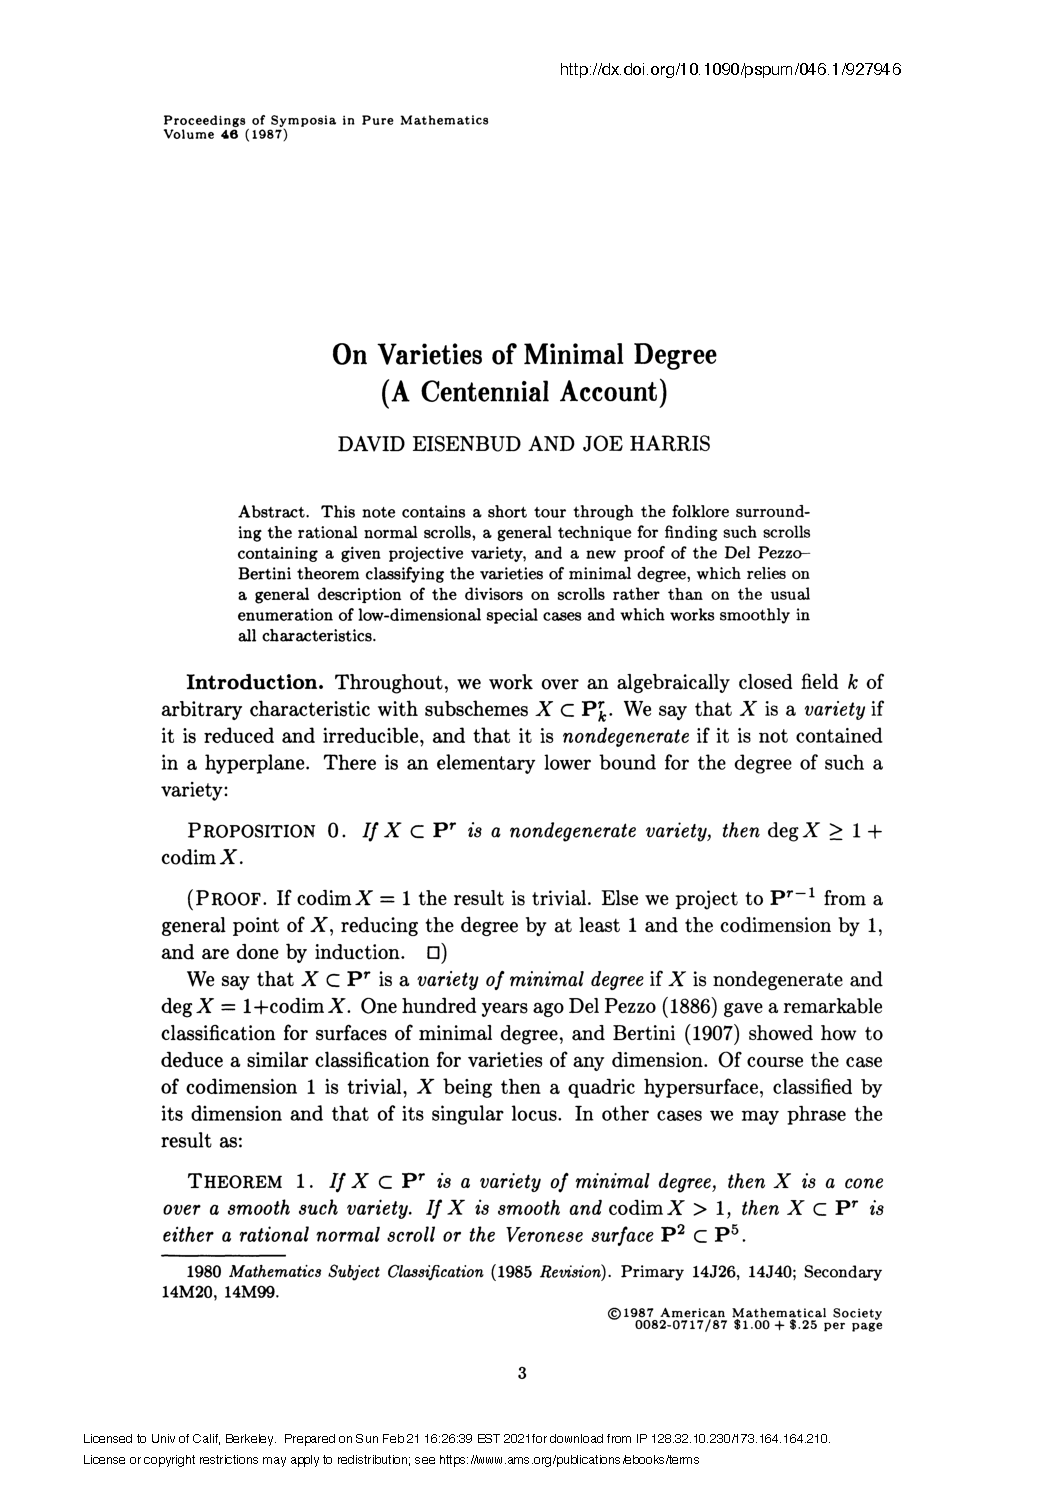
\includepdf[pages=1-11]{Centennial.pdf}


%footer for separate chapter files

\ifx\whole\undefined
%\makeatletter\def\@biblabel#1{#1]}\makeatother
\makeatletter \def\@biblabel#1{\ignorespaces} \makeatother
\bibliographystyle{msribib}
\bibliography{slag}

%%%% EXPLANATIONS:

% f and n
% some authors have all works collected at the end

\begingroup
%\catcode`\^\active
%if ^ is followed by 
% 1:  print f, gobble the following ^ and the next character
% 0:  print n, gobble the following ^
% any other letter: normal subscript
%\makeatletter
%\def^#1{\ifx1#1f\expandafter\@gobbletwo\else
%        \ifx0#1n\expandafter\expandafter\expandafter\@gobble
%        \else\sp{#1}\fi\fi}
%\makeatother
\let\moreadhoc\relax
\def\indexintro{%An author's cited works appear at the end of the
%author's entry; for conventions
%see the List of Citations on page~\pageref{loc}.  
%\smallbreak\noindent
%The letter `f' after a page number indicates a figure, `n' a footnote.
}
\printindex[gen]
\endgroup % end of \catcode
%requires makeindex
\end{document}
\else
\fi



